\documentclass[tikz]{standalone}
\usepackage{verbatim}
\usepackage{tikz}

\usetikzlibrary{plotmarks}
\usetikzlibrary{snakes}
\usetikzlibrary{arrows,positioning} 

\begin{document}
	\tikzset{
		>=stealth',
		punkt/.style={
			rectangle,
			rounded corners,
			draw=black, very thick,
			text width=6.5em,
			minimum height=2em,
			text centered},
		pil/.style={
			->,
			thick,
			shorten <=2pt,
			shorten >=2pt,},
		axis/.style={thick, ->, >=stealth'},
		important line/.style={thick}
	}
	
	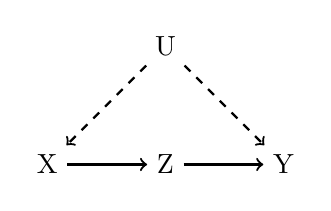
\begin{tikzpicture}
		\path (0, 0)      node (x)  {X}
		      (1.5, 0)    node (z)  {Z}
		      (3, 0)      node (y)  {Y}
		      (1.5, 1.5)  node (u)  {U};
		
		\draw[->, thick] (x) -- (z);
		\draw[->, thick] (z) -- (y);
		\draw[->, dashed, thick] (u) -- (y);
		\draw[->, dashed, thick] (u) -- (x);
	\end{tikzpicture}
\end{document}